% IEEE standard conference template; to be used with:
%   spconf.sty  - LaTeX style file, and
%   IEEEbib.bst - IEEE bibliography style file.
% --------------------------------------------------------------------------

\documentclass[letterpaper]{article}
\usepackage{spconf,amsmath,amssymb,graphicx,paralist,url}
\usepackage[utf8]{inputenc} 			% Zeichensatz
\usepackage[T1]{fontenc} 			% Umlaute unterstützen
\usepackage{float}
\usepackage[skip=3px]{caption}
\usepackage[boxed,vlined,linesnumbered]{algorithm2e}	% Pseudocode
\SetAlCapSkip{2ex}				
% \setalcapskip{2ex}							% caption unter code
\hyphenation{now-list}
\hyphenation{later-list}

% Example definitions.
% --------------------
% nice symbols for real and complex numbers
\newcommand{\R}[0]{\mathbb{R}}
\newcommand{\C}[0]{\mathbb{C}}

% bold paragraph titles
\newcommand{\mypar}[1]{{\bf #1.}}

% Title.
% ------
\title{Parallel implementation of Fringe Search}
%
% Single address.
% ---------------
\name{Lukas Mosimann, Christian Zeman} 
\address{ETH Z\"urich\\Z\"urich, Switzerland}

% For example:
% ------------
%\address{School\\
%		 Department\\
%		 Address}
%
% Two addresses (uncomment and modify for two-address case).
% ----------------------------------------------------------
%\twoauthors
%  {A. Author-one, B. Author-two\sthanks{Thanks to XYZ agency for funding.}}
%		 {School A-B\\
%		 Department A-B\\
%		 Address A-B}
%  {C. Author-three, D. Author-four\sthanks{The fourth author performed the work
%		 while at ...}}
%		 {School C-D\\
%		 Department C-D\\
%		 Address C-D}
%

\begin{document}
%\ninept
%
\maketitle
%

\begin{abstract}
We've implemented and parallelized Fringe Search, a single-pair shortest path algorithm, for a shared memory environment. By already using two cores, the parallel version outperformed the sequential one on our benchmark graphs without showing any noticeable compromises in terms of path quality.
\end{abstract}

\section{Introduction}\label{sec:intro}

This project was part of the course \textit{Design of Parallel and High-Performance Computing} given by Torsten Hoefler and Markus Püschel in autumn 2013 at ETH Zürich.


\mypar{Motivation} 
Pathfinding is an important problem occurring in many applications, especially in computer games and robotics. Finding the shortest path between two specific nodes is a pathfinding problem tackled by algorithms such as A* or Fringe Search. Unlike A*, Fringe Search doesn't assure finding the shortest path (rather a path "short" enough) but it usually outperforms A* as shown in \cite{fringe:05}.\\
In \cite{brand:09} Fringe Search has been implemented to run in parallel on a distributed memory environment. The goal of this paper was the implementation of a fast parallel Fringe Search for a shared memory environment.

\mypar{Related work} This paper is mainly based on three papers. The Fringe Search algorithm has been introduced in \cite{fringe:05}. S. Brand and R. Bidarra have implemented a parallel version in a distributed memory environment, published in \cite{brand:09} and in \cite{brand:12}. For this paper, the implementation has been done for a shared memory environment.

\section{Background: Shortest Path Problem}\label{sec:background}
In this section we define the single-pair shortest path problem and introduce two algorithms that are used to solve it.

\mypar{Single-pair shortest path problem}
A problem where the goal is to find the shortest path between a given start and an end node in a directed or undirected graph.

\mypar{A*}
A very popular algorithm that uses a best-first search approach for solving the single-pair shortest path problem. For the best-first search it uses a heuristic function that estimates the distance to the end node. It always finds the shortest possible path as long as the heuristic function never overestimates the real distance. We say the found path is "optimal". A* uses a priority queue for selecting the next best node what causes each insertion into the queue having complexity $\mathcal{O}(\log n)$ with respect to the size of the queue.

\mypar{Fringe Search}
Another single-pair shortest path algorithm that is similar to A*, but instead of a priority queue that always has the most promising reachable node first it stores the reachable nodes in a doubly linked list where an insertion has only complexity $\mathcal{O}(1)$. It visits a node if it's "promising enough" which is determined by a global threshold value that will be continuously increased. By doing this, the path will not be optimal but the algorithm is usually faster than A*, as shown in \cite{fringe:05}. See figure~\ref{fig:algo} for an example.
\begin{figure}[h]\centering
  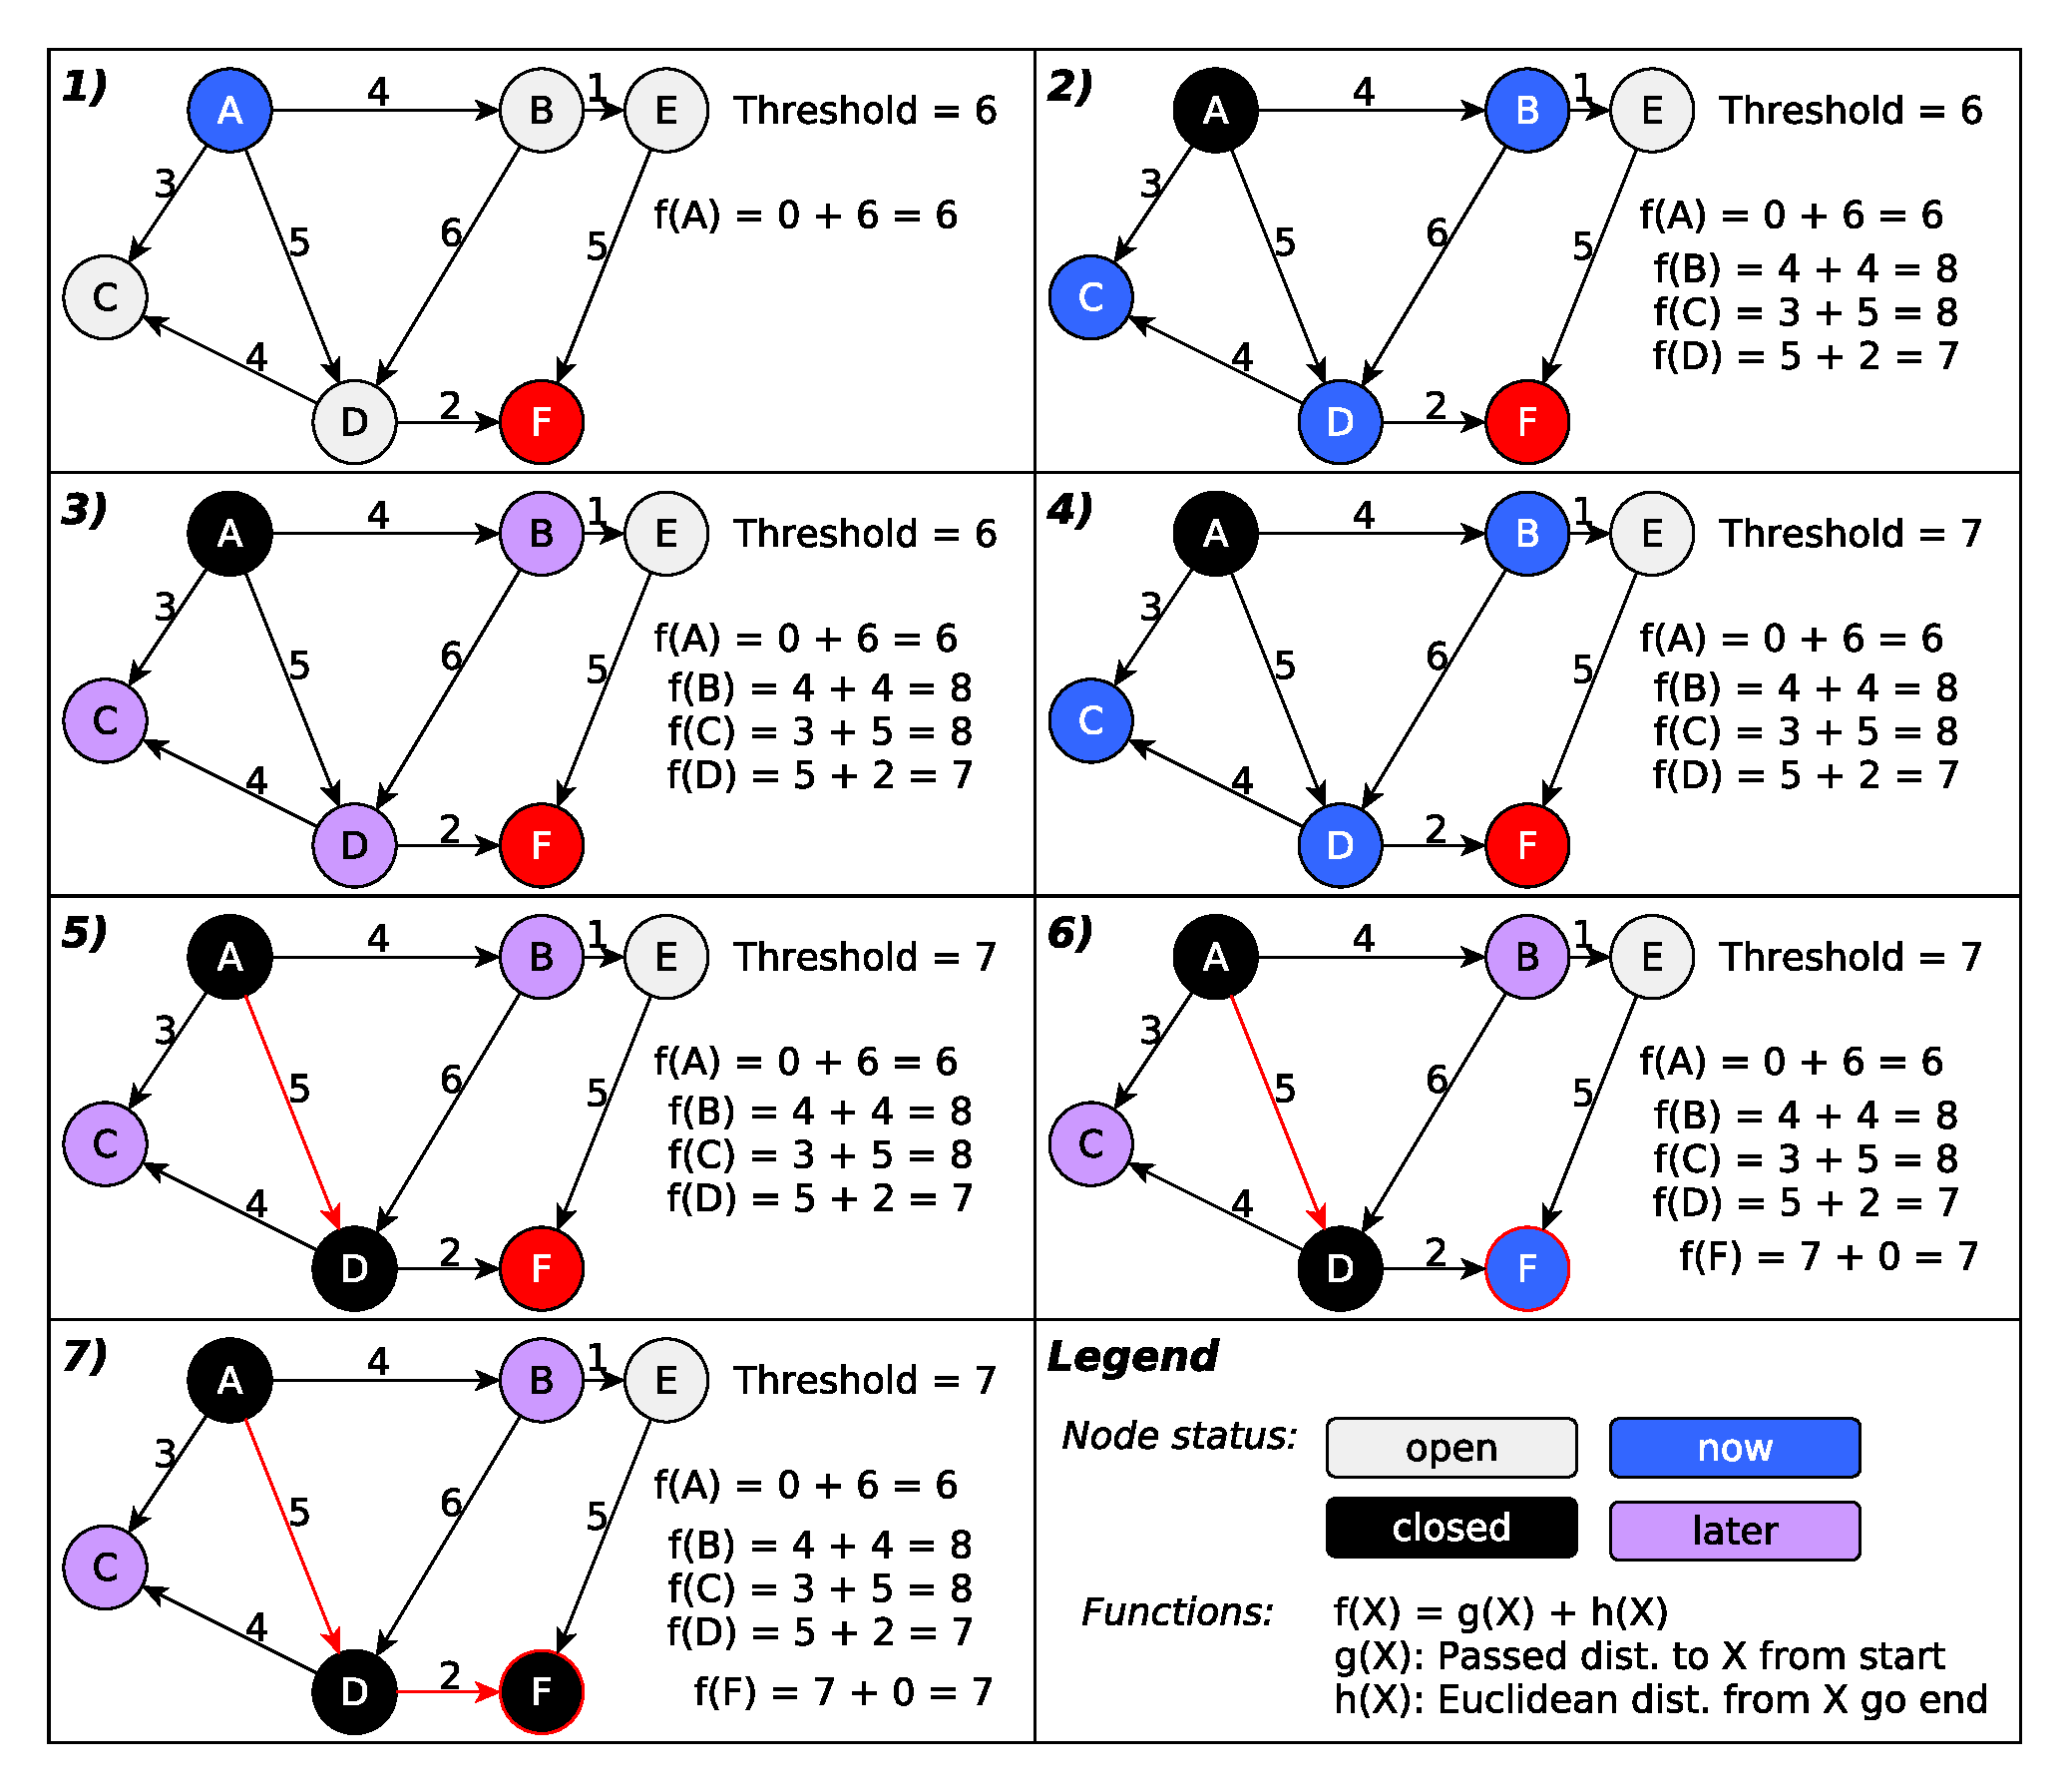
\includegraphics[scale=0.245]{fringe_rep.eps}
  \caption{Fringe Search example; start = A, end = F \label{fig:algo}}
\end{figure}


\section{Concept and implementation}\label{sec:impl}

In this section we give an overview of the implementation, emphasize important aspects and illustrate the used concepts for locking. 

\subsection{Language and data structures}\label{ssec:lang}

All implementations have been done with C++11, OpenMP 3 and some inline assembly for the locks.

\mypar{Graph structure}
We use a directed graph implemented as adjacency list. This means that each node stores a list of pointers to its neighbours as well as the distance to these nodes. Basically, this distance can be everything as long as there exists a good heuristic cost function that does not overestimate the real distance. \\
In our experiments we interpreted the graph as nodes in a 2D plane, mainly for visualization purposes. Every node has a position so we can use the Euclidean distance as our heuristic function (e.g. one could also use the Manhattan distance).

\mypar{Status of a node} Each node possesses one of the following states:
\begin{compactitem}
\item \textit{Inactive:} The node has not yet been visited. In the beginning each node except the start node is inactive.
\item \textit{Closed:} The node has been visited and its cost (sum of real distance from start to this node and the estimated distance from this node to the end) is below the current threshold. A closed node won't be updated anymore.
\item \textit{Now:} The node has a closed neighbor, what means that we know the real distance from the start to this node. We don't know yet if the cost of this node is below or above threshold.
\item \textit{Later:} Also a node with a closed neighbor, but the cost of this node is known and above the threshold. The node won't be visited until we increase the threshold or find a better path to it.
\end{compactitem}

\mypar{Linked lists}
We use two doubly linked lists we will henceforth call the \textit{nowlist} and the \textit{laterlist}. The nowlist contains the nodes that have status \textit{now} whereas the laterlist contains the nodes with status \textit{later}. Whenever the nowlist becomes empty we increase the threshold and swap the two lists as we also swap the definition of the states (now will become later and vice versa). 

\subsection{From sequential to parallel}\label{ssec:seqpar}

First, we implemented a strictly sequential Fringe Search in order to have a basis for the parallel implementation and also as a reference for the benchmarks regarding the speedup of the parallel version. The pseudocode for Fringe Search can be found in algorithm \ref{algo:par}.

\mypar{Parallel Fringe Search}
Besides the necessary locks for the insertion and removal from the lists, the threshold relaxation part (see lines \ref{code:thresh}-\ref{code:swap} in algorithm \ref{algo:par}) is the bottleneck, because this part has to be done sequentially by only one thread and not before all threads reached this point.

\begin{algorithm}[t!]
\SetKwFunction{heuristicDist}{heuristicDist}
\SetKwFunction{reconstructPath}{reconstructPath}
\SetKw{oder}{ or }

\SetInd{0.5em}{0.5em}
\newcommand{\var}[1]{{\textit{#1}}}

add node \var{start} to \var{nowlist} \;
$\var{laterlist} \gets \emptyset$ \;
$\var{threshold} \gets \heuristicDist{\var{start}, \var{end}}$ \;
\While{$\var{nowlist} \neq \emptyset \oder \var{laterlist} \neq \emptyset $}{ 
	\While(\tcp*[f]{\textnormal{$\exists$ nodes $\leq$ \var{threshold}}}){$nowlist \neq \emptyset$}{
		\var{x} $\gets$ Node from \var{nowlist} \;
 		\eIf{$\var{x}.\var{distanceEstimation} \leq \var{threshold}$}{
 	 		\If{$\var{x}$ = $\var{end}$}{
				\Return $\reconstructPath{}$ \tcp*[f]{\textnormal{done}}
	 		}
 			$\var{x}.\var{status} \gets closed$ \;
			\ForEach{\textnormal{neighbour} $\var{nb}$}{
				\uIf{$\var{nb}.\var{status}$ = $ \var{now}$}{
					calculate new distance estimation \var{dist} \;
					\If{$\var{dist} < \var{nb}.\var{distanceEstimation}$}{
						$\var{nb}.\var{distanceEstimation} \gets \var{dist}$ \;
						$\var{nb}.\var{parent} \gets \var{x} $\;
						move $\var{nb}$ right behind $\var{x}$ in $\var{nowlist}$ \;
					}
				}
				\uElseIf{$\var{nb}.\var{status} = \var{later}$}{
					calculate new distance estimation \var{dist} \;
					\If{$\var{dist} < \var{nb}.\var{distanceEstimation}$}{
						$\var{nb}.\var{distanceEstimation} \gets \var{dist}$ \;
						$\var{nb}.\var{parent} \gets \var{x} $\;
						remove $\var{nb}$ from $\var{laterlist}$ \;					
						insert $\var{nb}$ right behind $\var{x}$ in $\var{nowlist}$ \nllabel{code:moveback}\;
						$\var{nb}.\var{status} \gets \var{now}$ \;
					}
				}
				\ElseIf{$\var{nb}.\var{status} = \var{inactive}$}{
					calculate $\var{nb}.\var{distanceEstimation}$ \;
					$\var{nb}.\var{parent} \gets \var{x}$\;
					insert $\var{nb}$ right behind $\var{x}$ in $\var{nowlist}$ \;
					$\var{nb}.\var{status} \gets \var{now} $ \;
				}
			}
			remove $\var{x}$ from $\var{nowlist}$ \;
		}{
			$\var{x}.\var{status} \gets \var{later}$\;
 			move $\var{x}$ into \var{laterlist} \nllabel{code:move}\;
 		}
	}
	increase $\var{threshold}$ \nllabel{code:thresh} \;
	swap $\var{nowlist} $ and $ laterlist$\nllabel{code:swaplist} \;
	swap the definition of $\var{now}$ and $\var{later}$ \nllabel{code:swap} \;
}
\Return \,-1 \tcp*[r]{\textnormal{no existing path to end}}
\caption{parallelizable Fringe Search with two lists\label{algo:par}}
\end{algorithm}

\mypar{Swapping the lists}
Whenever we relax the threshold, the nowlist/laterlist and the states of the included nodes will get swapped (lines \ref{code:swaplist} and \ref{code:swap} in algorithm \ref{algo:par}), as the nodes with status later are potentially below the threshold after increasing it.\\
After swapping the lists  we don't want to have all the threads starting from the first node in the nowlist, but rather have them distributed over the whole nowlist. We achieve this by remembering the last visited node in the laterlist for each thread (e.g. we save the last node moved into the laterlist at line \ref{code:move} in algorithm \ref{algo:par}). By doing this, the thread can start from this node after swapping the lists and we get the wanted distribution. Another advantage of this behavior is that we might profit from the cache effect, because this node might still be in the cache.\\
But of course we have to check if this node truly is in the nowlist which can't be guaranteed (a node remembered at line \ref{code:move} could have been moved back at line \ref{code:moveback}). If it's no longer there we just start from the first node in the nowlist.

\subsection{Locking}\label{ssec:lock}

\mypar{Traversing the list}
Whenever a thread traverses the nowlist it tries to lock every node it encounters. But instead of forcing a lock, it just tries to lock the node and if it's successful it can work with this node (visit the adjacent nodes, etc.). If the thread fails trying to lock the node, this means that another thread is working with exactly this node.\\
In case of a unsuccessful try we don't go to the very next node in the list, because the thread currently holding the lock will most likely try to lock the next node soon and like this the two threads would block each other quite often. Instead, we skip a few nodes in order to achieve a nice distribution of the threads over the nowlist.\\
Skipping 150 nodes has proven to provide a relatively good distribution that results in a faster runtime for large graphs (more than $10^6$ nodes).

\mypar{Lock type}
Next to the locking mechanism provided by OpenMP we've implemented the following locks
\begin{compactitem}
\item TAS: test-and-set lock
\item TAS EXP: TAS with exponential back-off
\end{compactitem}
by using inline assembly.

\mypar{Avoiding deadlocks}
%TODO: esch das do wörkli klar? Has afe chli gänderet, aber bemr noni ganz sechr :) v.a. de erst absatz esch no schwerig...
In order to avoid deadlocks we lock nodes always in the same order. This means we lock from right to left in both lists and we first lock the nodes in the nowlist, and then the nodes in the laterlist (see figure~\ref{fig:lock}).\\
This requires that we know the relative location of the nodes we would like to lock (i.e. node X is left of node Y). This is always the case except for one situation:\\
Let's say we've locked node A in the nowlist and via this node we find a shorter path to an adjacent node B, that is already in the nowlist and below threshold. In this case we would like to update B's cost, its parent node (A will become parent node of B) and move it right behind A. For all this we require a lock on B, but we can't tell if B is left or right of A, because we got to this node via a pointer in the adjacency list of A. If we now forced a lock on B we could run into a deadlock because it's possible that another thread has locked B and, as its cost is already below threshold, is waiting for the lock on A, since it's an adjacent node of B.\\
The solution of this problem is to not force a lock but instead, just trying to lock the adjacent node. If the try is successful we can update the path and move it. If the try was not successful we just leave the old path that was already below threshold. This does not change the characteristic of the algorithm since the adjacent node could have already been closed by another thread as its value is below threshold. \\
Locking a node that is not in any of our two lists can be done without any problems because no thread will ever try to lock more than one node outside the lists.\\
Acting as described above, we prevent any possible circular wait dependencies and so no deadlocks can occur \cite{Coffman:71}.

\begin{figure}[h]\centering
  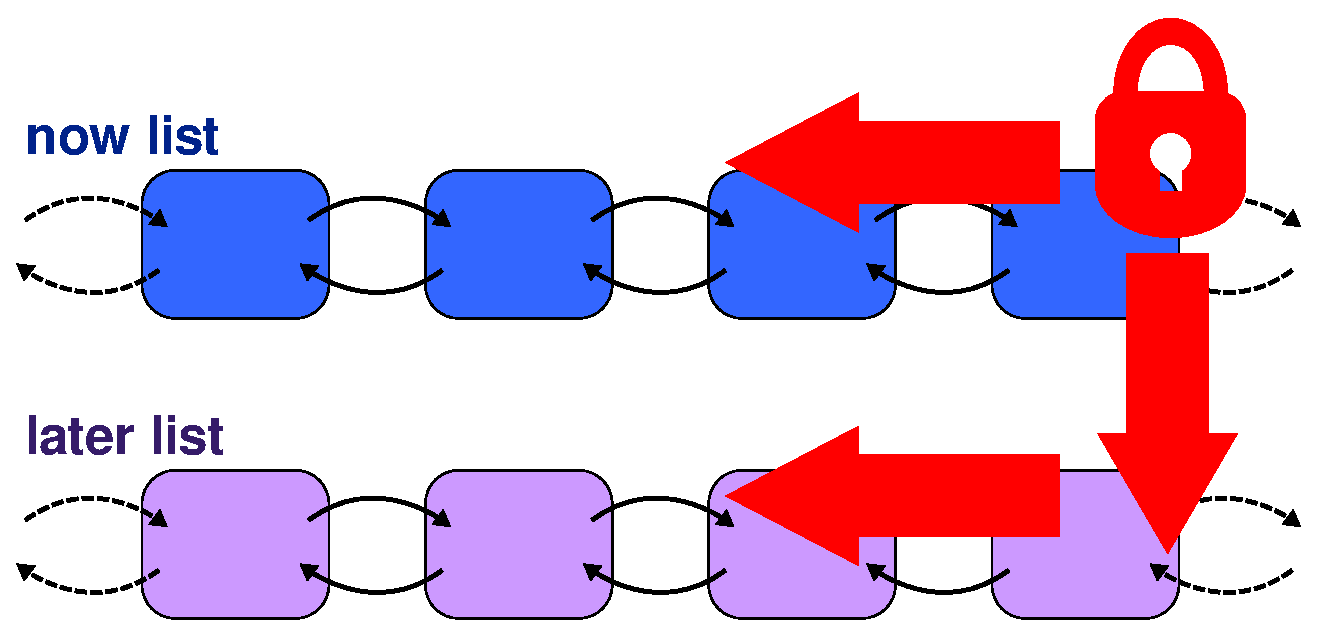
\includegraphics[scale=0.38]{locking.eps}
  \caption{Locking direction \label{fig:lock}}
\end{figure}

\mypar{Inserting nodes}
The sequence for inserting nodes into a list is shown in figure~\ref{fig:insert}.

\begin{figure}[h]\centering
  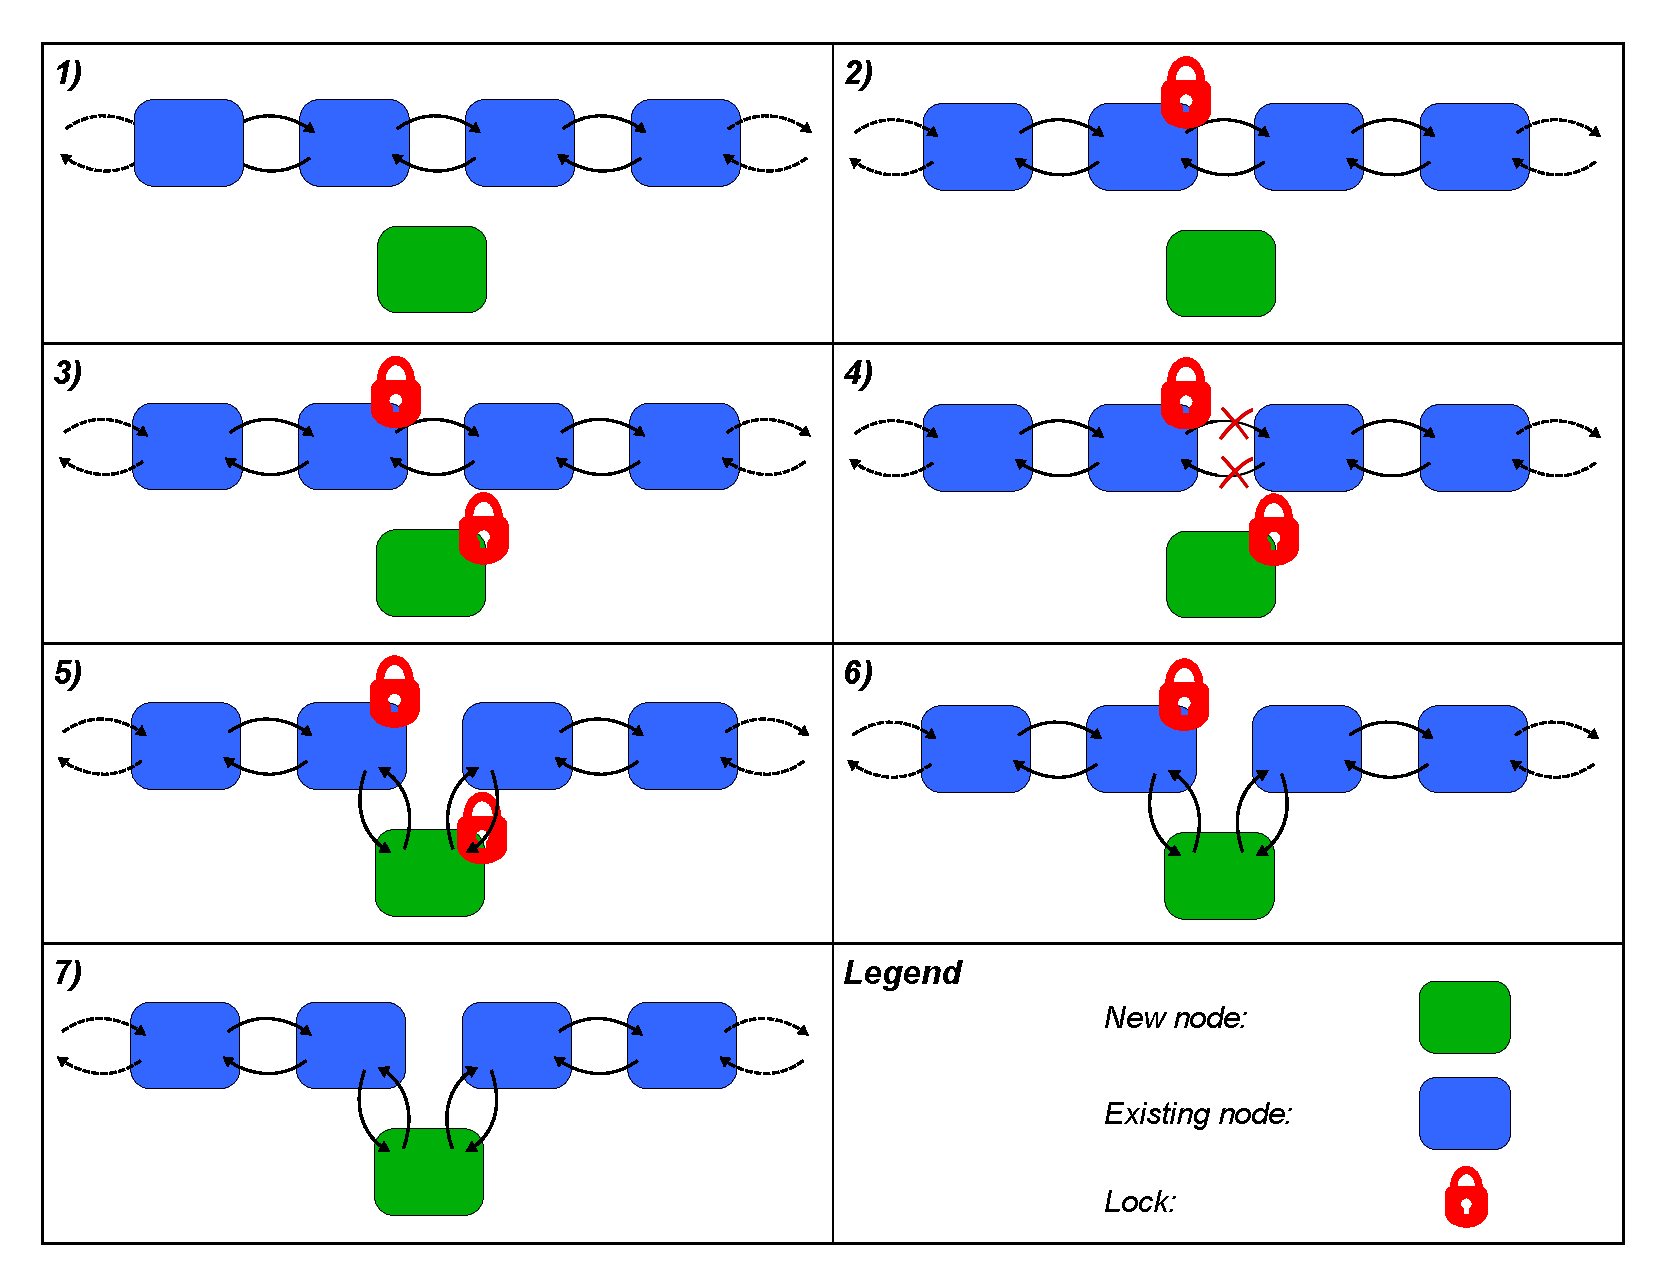
\includegraphics[scale=0.31]{insert.eps}
  \caption{Insert a node into the list \label{fig:insert}}
\end{figure}

\mypar{Removing nodes}
The sequence for physically removing nodes from a list is shown in  figure~\ref{fig:remove}. We've implemented and tested the removal with two different approaches. The first approach is to physically remove the node immediately as shown in figure~\ref{fig:remove}. The second one is to just mark it as removed, go on, and let other threads physically remove it while they are traversing the list (lazy deletion).

\mypar{Acquiring locks}
All locks are acquired by "optimistic locking". So if we try to get locks on nodes with specific properties (e.g. the node must be predecessor of another node or the node must have a specific state), we spin/wait until we get the lock and after acquiring the lock we ensure the conditions are still true. If not, we release the lock immediately.

\begin{figure}[h]\centering
  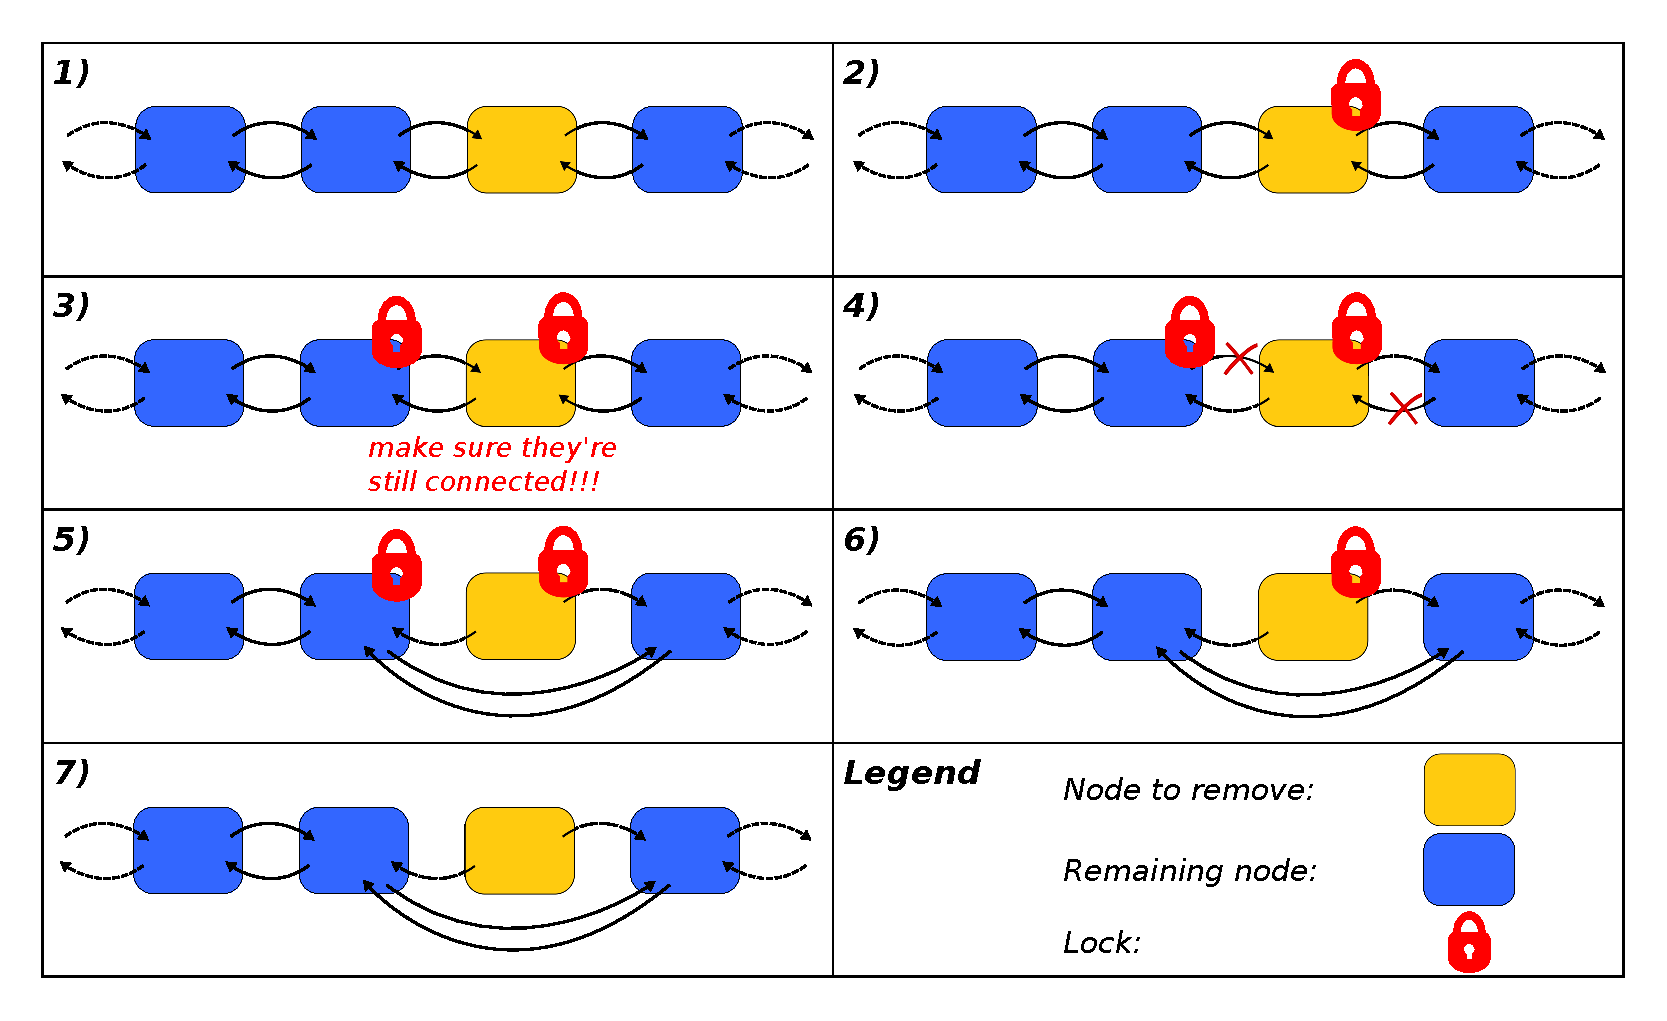
\includegraphics[scale=0.31]{remove.eps}
  \caption{Remove a node from the list. Note: The pointers of a removed node remain in place so that a traversing thread won't get lost. \label{fig:remove}}
\end{figure}



\section{Experimental Results}\label{sec:exp}

In this section we evaluate our implementation in terms of the speed of the sequential algorithm, the performance of the different locks, strong scaling, weak scaling, and several properties of the algorithm depending the threshold relaxation parameter.

\subsection{Experimental setup}\label{ssec:setup}

\mypar{Hardware and compiler}
The experiments have been done on kanifushi.inf.ethz.ch:
\begin{compactitem}
\item NUMA model with 32 CPUs on 4 nodes
\item 8 CPUs per node
\item Intel(R) Xeon(R) CPU E7- 4830 @ 2.13GHz
\item per CPU: 32KB L1 cache, 256KB L2 cache
\item per node: 24MB L3 cache, 16GB memory
\end{compactitem}
We've only used 1 node with 8 CPUs as the implementation has been done for a shared memory environment. To enforce this, the application had to be executed with the \textit{numactl} tool (e.g. \textit{numactl -{}-cpunodebind=0 -{}-membind=0 fringe}). The code has been compiled with g++ v. 4.6.1 using O1 optimization. All of the following performance analysis plots are the result of 50 runs on 1 node.

\mypar{Graphs used for benchmarking}
Each experiment has been run using two graph types with different obstacles, the "Cross Graph" and the "Circle Graph" which are illustrated in figure~\ref{fig:graphs}. Both graphs have the following properties:
\begin{compactitem}
\item based on a regular grid with distance 1
\item 8 edges per node (except at the border)
\item each node is displaced randomly according to a normal distribution with $\sigma = 0.3$
\item start node is top left and end node is bottom right
\end{compactitem}

\begin{figure}[h]\centering
  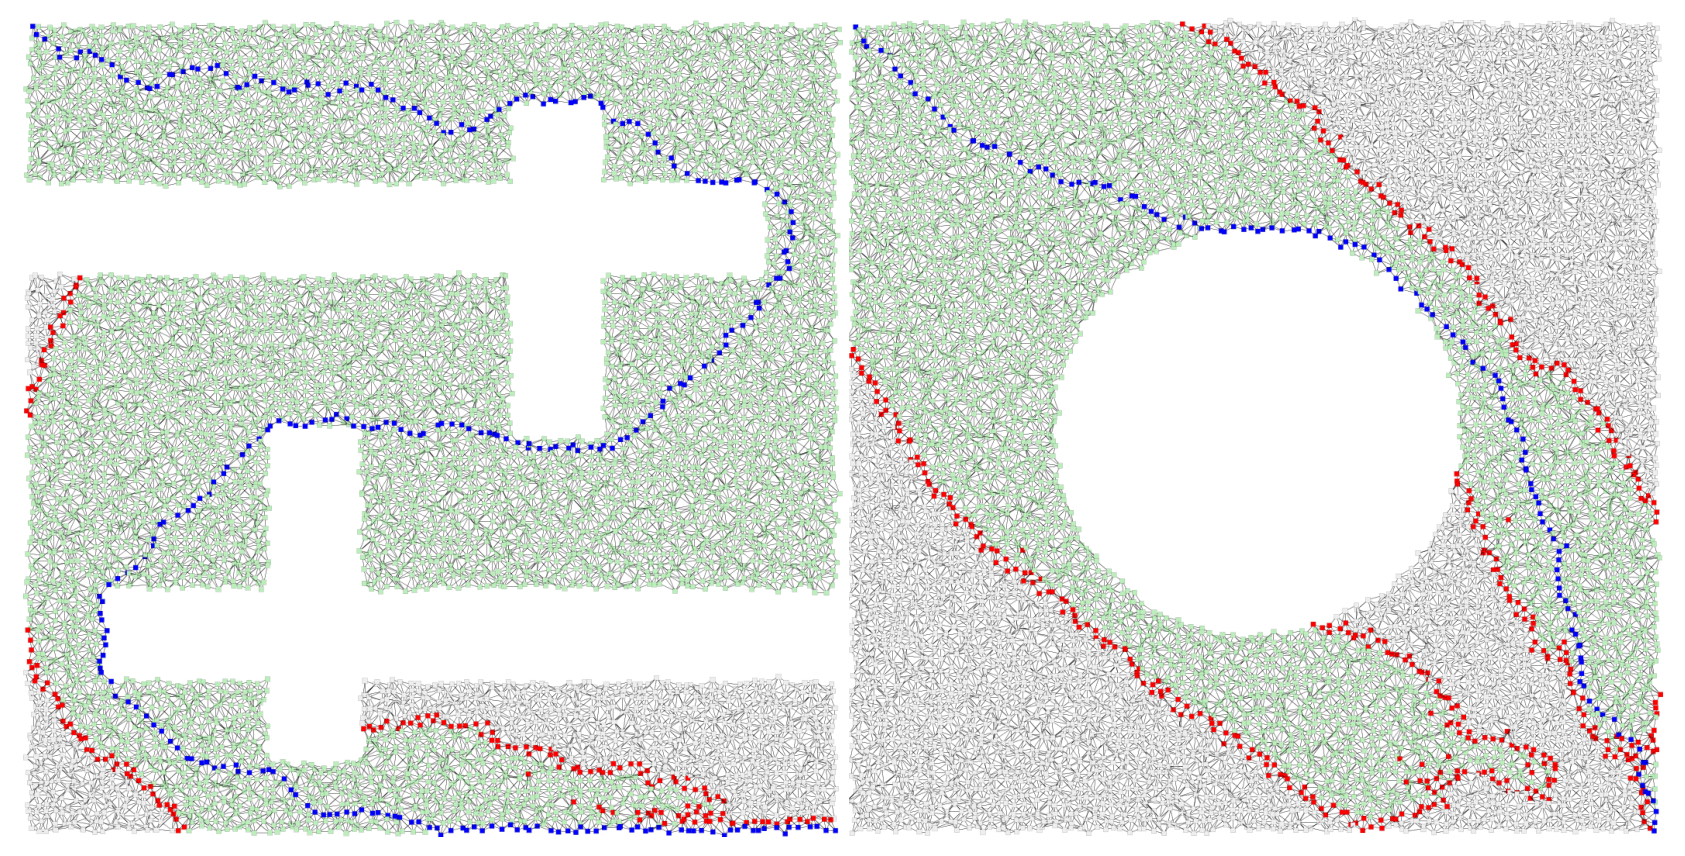
\includegraphics[scale=0.3]{benchmark_graphs.eps}
  \caption{The graphs used for benchmarking: "Cross Graph" (left) and "Circle Graph" (right). The blue nodes represent the found path, the green nodes are "closed" and the red nodes have status "now" or "later". \label{fig:graphs}}
\end{figure}

\subsection{Results}\label{ssec:results}

\mypar{Sequential Fringe Search}
In order to affirm good performance of the sequential version, we tested the sequential Fringe Search against the A* search from the Boost Graph, Library\footnote{\url{http://www.boost.org/doc/libs/1_55_0/libs/graph/doc/index.html}} as we couldn't find a reliable implementation of Fringe Search we could compare our code to.\\
Our implementation of Fringe Search proved to be much faster than A* from the Boost Graph Library (about 10 times as fast on a graph with $1024 \times 1024$ nodes and a threshold relaxation value of $1$). But of course, one has to take into account that Fringe Search doesn't guarantee an optimal path like A* does.

\mypar{Locks}
The locks we've implemented with inline assembly (see section \ref{ssec:lock}) were significantly faster than the locks provided by OpenMP (see figure~\ref{fig:lock_bench}). Thus, we used the test-and-set lock with exponential back-off for our implementation. The following benchmarks are all based on the implementation with these locks.

\begin{figure}[h]\centering
  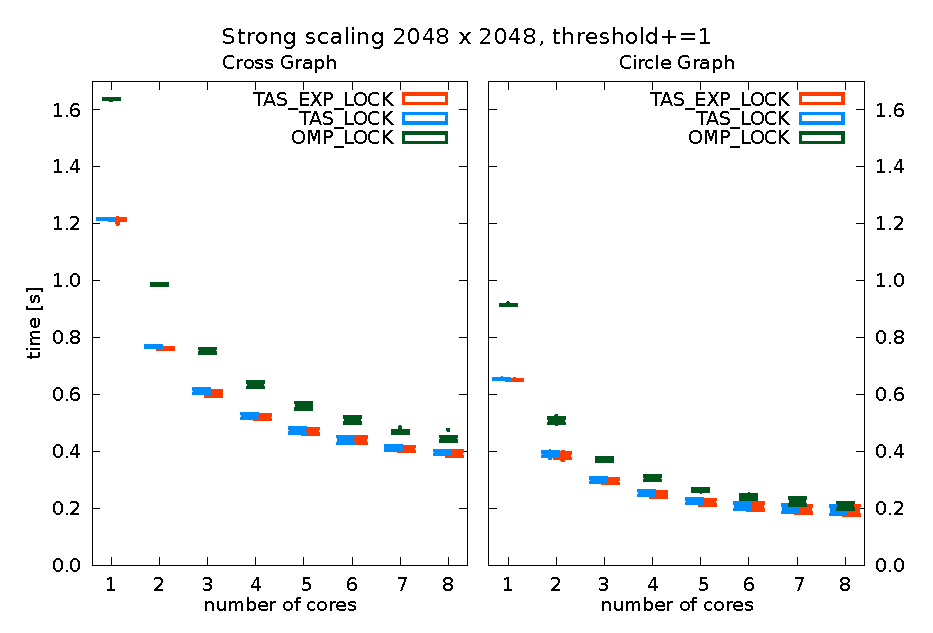
\includegraphics[scale=0.558]{lock_benchmark.eps}
  \caption{Strong scaling using different locks.\label{fig:lock_bench}}
\end{figure}


\mypar{Strong scaling}
One of the most important questions is how much faster the application gets by using more cores for a fixed problem size. The results are shown in figure~\ref{fig:strong_scaling}.
\begin{figure}[h]\centering
  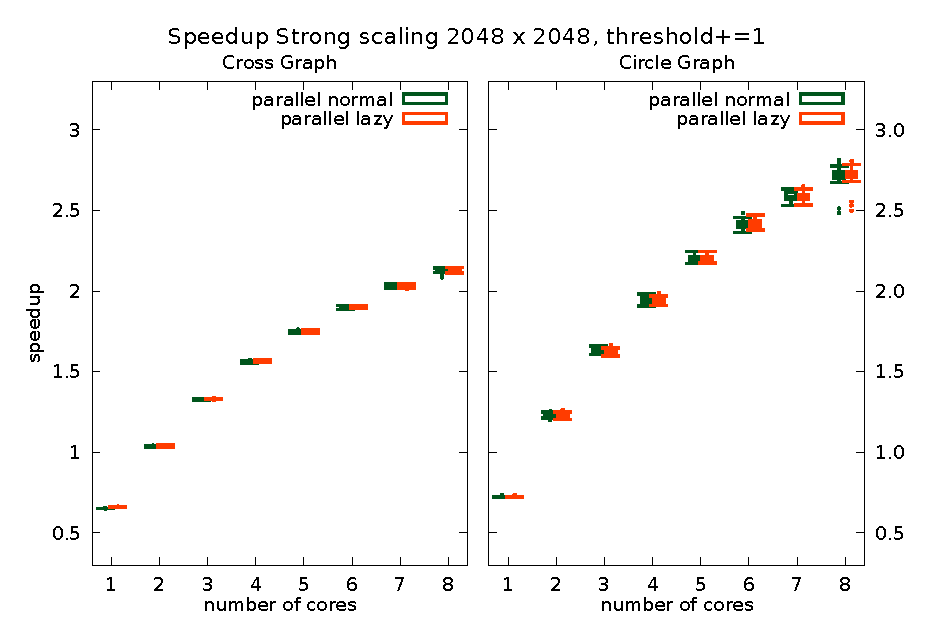
\includegraphics[scale=0.558]{strong_scaling_speedup.eps}
  \caption{Strong scaling (speedup against sequential version) \label{fig:strong_scaling}}
\end{figure}
For both benchmark graphs the parallel version is faster than the sequential version if it uses two or more cores.

\mypar{Weak scaling}
Because of the limitations in terms of speedup according to Amdahl's law (also visible in figure~\ref{fig:strong_scaling}), the next question is how the runtime behaves for an increasing problem size while keeping the problem size per core (number of nodes per core) constant.
\begin{figure}[h]\centering
  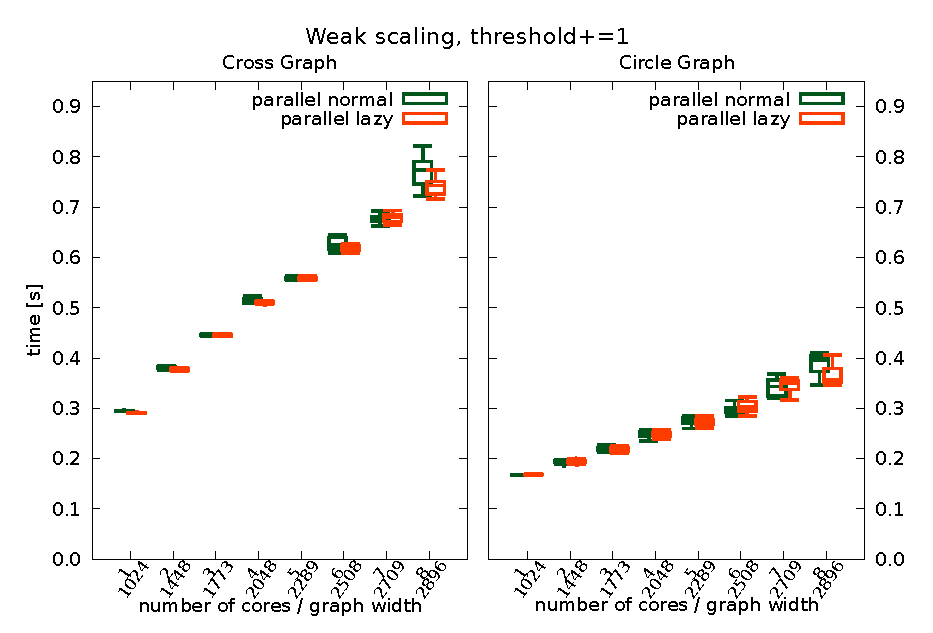
\includegraphics[scale=0.558]{weak_scaling.eps}
  \caption{Weak scaling\label{fig:weak_scaling}}
\end{figure}\\
As shown in figure~\ref{fig:weak_scaling}, we still experience an increase in runtime with increasing problem size but it's not that much and the behavior actually meets our expectations, because with increasing problem size we also increase the time the program spends in the sequential part (longer path will lead to more threshold updates). Since the shortest path in the Circle Graph is shorter than the one in the Cross Graph, we need less threshold updates and so the time does not increase as much as for the Cross Graph.

\mypar{Normal versus lazy removal} Looking at the figures~\ref{fig:strong_scaling} and \ref{fig:weak_scaling}, it's apparent that it doesn't matter which approach for removing the nodes we use (lazy vs. normal, see section \ref{ssec:lock}). The difference in speed is negligible. Therefore we will only show the results for normal removal in future plots.

\mypar{Path length versus $\#$ cores}
An interesting question is if the path length gets worse the more threads we have. As mentioned in section \ref{ssec:lock} (avoiding deadlocks) we cannot always update a node with a better path if it's already below threshold and locked by another thread. And the more threads we have the higher is the possibility that this happens.
\begin{figure}[h]\centering
  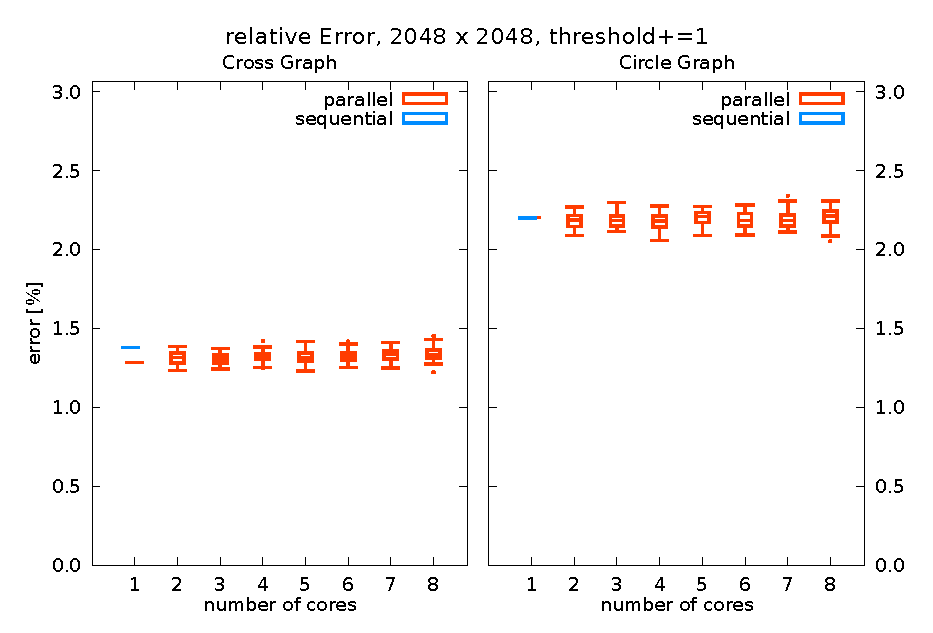
\includegraphics[scale=0.558]{error_cores.eps}
  \caption{Relative error in path length compared to A* depending on the number of cores\label{fig:error_cores}}
\end{figure}
As shown in figure~\ref{fig:error_cores} the number of cores/threads does not affect the quality of the path.

\mypar{Path length versus threshold relaxation}
The threshold relaxation value defines by how much we increase the threshold once the nowlist is empty. If we increase the threshold by a small value we will just consider few new nodes, but they all are relatively promising nodes resulting in a short path. If we increase the threshold by a bigger value we'll have more nodes to look at, but not all of them will be that good in terms of path length.
\begin{figure}[h]\centering
  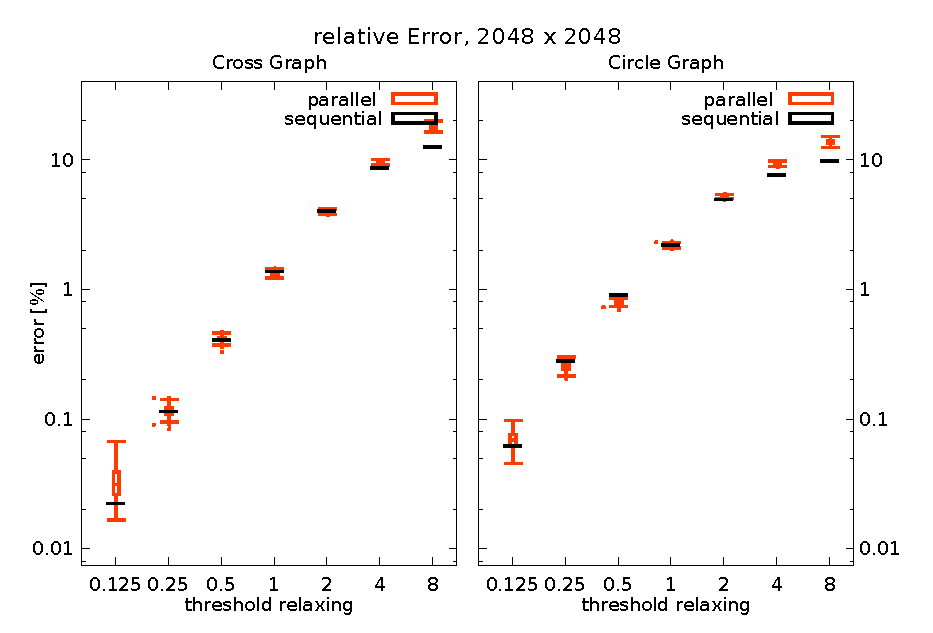
\includegraphics[scale=0.558]{error_threshold.eps}
  \caption{Relative error in path length compared to shortest path (A*) depending on threshold relaxation value\label{fig:error_thresh}}
\end{figure}
As you can see in figure~\ref{fig:error_thresh}, the relative error gets quite high once we have a threshold relaxation value greater than 1, whereas the path quality is very good for small threshold relaxation values.

\mypar{Runtime versus threshold relaxation}
According to figure~\ref{fig:error_thresh}, a low threshold relaxation value leads to a short path. However, by doing this we always just have a few nodes in our nowlist, so the different threads will have more collisions and we have to increase the threshold more often which means that we will spend more time in the sequential part of the algorithm. Therefore we expect our algorithm to be slower with smaller the threshold relaxation values. As it can be seen in figure~\ref{fig:runtime_thresh}, this is the case.\\
\begin{figure}[h]\centering
  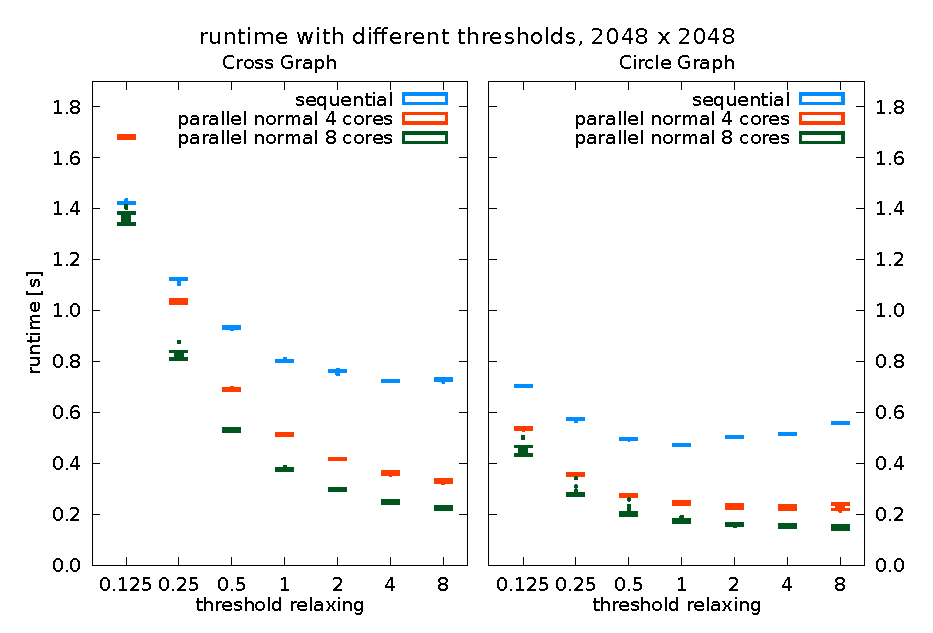
\includegraphics[scale=0.558]{runtime_threshold.eps}
  \caption{Runtime depending on threshold relaxation value\label{fig:runtime_thresh}}
\end{figure}
Another interesting aspect of figure \ref{fig:runtime_thresh} is that the sequential version gets slower for very high relaxation values. This is due to the fact that high thresholds at the start will lead to a relatively big fan-out (compare with figure~\ref{fig:graphs}) which one core alone won't be able to handle in sufficient time. More cores can handle this relatively big nowlist more efficiently and, as shown in figure~\ref{fig:speedup_thresh}, the turnaround is later.
\begin{figure}[h]\centering
  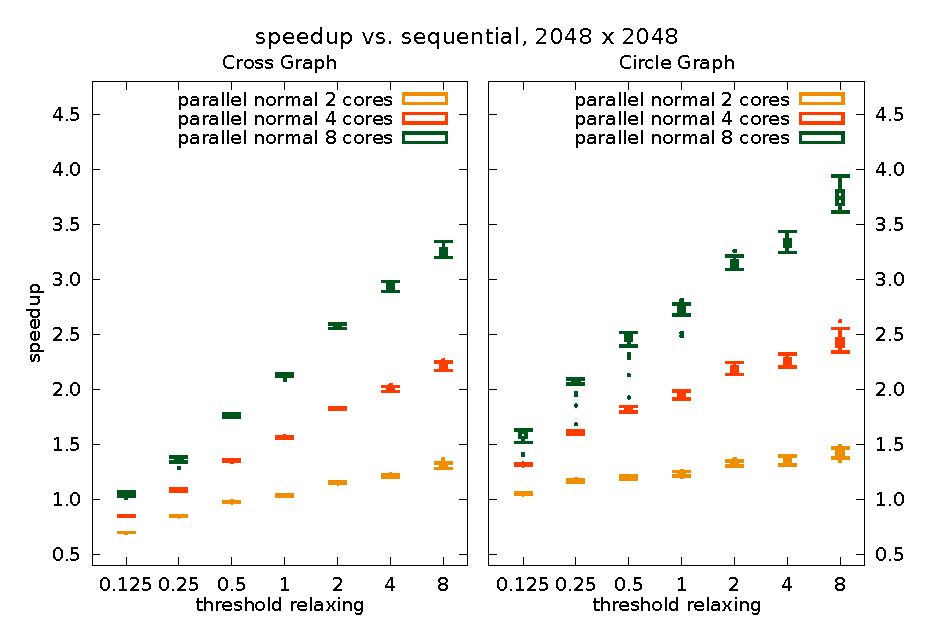
\includegraphics[scale=0.558]{speedup_threshold.eps}
  \caption{Speedup of parallel version versus sequential version using different threshold relaxation values\label{fig:speedup_thresh}}
\end{figure}


\section{Conclusions}

We've implemented a sequential version of Fringe Search that is significantly faster than the A* implementation from the Boost Graph Library. Then we've parallelized it for a shared memory environment. The important results are:
\begin{itemize}
\item The parallel version running on only two cores was already faster than the sequential version.
\item The parallel version didn't have any noticeable compromises in terms of path quality.
\item Strong scaling has shown to be quite good, but of course limited by having a sequential part in the algorithm.
\item Weak scaling is good but not perfect due to the increasing sequential part with increasing graph size.
\item The implementation can be tuned with the threshold relaxation parameter in order to meet the individual requirements concerning path quality and runtime.
\end{itemize}
There is still a significant sequential part which is increasing with the problem size (threshold relaxation and list swapping) that can't be avoided easily, but nevertheless we believe that this is a relatively fast implementation on a shared memory environment.\\
Next steps could be enhancing the application to make it also work in a distributed/hybrid memory environment.



% References should be produced using the bibtex program from suitable
% BiBTeX files (here: bibl_conf). The IEEEbib.bst bibliography
% style file from IEEE produces unsorted bibliography list.
% -------------------------------------------------------------------------
\bibliographystyle{IEEEbib}
\bibliography{bibl_conf}

\end{document}


